\documentclass[11pt]{article}
\usepackage[a4paper,margin=2.4cm]{geometry}
\usepackage{amsmath,amssymb}
\usepackage{booktabs}
\usepackage{float}
\usepackage{graphicx}
\usepackage{enumitem}
\usepackage{microtype}
\usepackage[hidelinks]{hyperref}
\setlist{itemsep=2pt,topsep=4pt}

\newcommand{\F}{\mathcal{F}}
\newcommand{\Fi}{\mathcal{F}^{-1}}
\newcommand{\x}{\mathbf{x}}
\newcommand{\OD}{\mathrm{OD}}
\DeclareMathOperator*{\argmax}{arg\,max}

\title{From burst to vessel graph:\\ stabilisation, optical density and Hessian vesselness}
\author{}
\date{11 October 2026}

\begin{document}
\maketitle

\noindent This note sets out the first stages of vessel annotation as equations: an unstabilised burst is
aligned by phase correlation and averaged (section~\ref{sec:stab}); the average is converted to optical density
(section~\ref{sec:od}); multi-scale Gaussian derivatives give the Hessian at every pixel and scale
(sections~\ref{sec:scale}--\ref{sec:hessian}), from which Frangi's vesselness and a width estimate follow
(sections~\ref{sec:frangi}--\ref{sec:width}); and vesselness is turned into a graph (section~\ref{sec:graph}).
Section~\ref{sec:limits} shows where this Hessian chain fails, which is why the later stages use oriented cells.

\section*{Notation}
\begin{tabular}{@{}ll@{}}
$I_k(\x)$, $k = 1,\dots,N$ & the frames of the burst; mono12, so values are DN in $[0, 4095]$ \\
$\x = (x, y)$ & pixel position; the image is $W \times H$ pixels \\
$M_k(\x) \in \{0, 1\}$ & validity mask of frame $k$ \\
$\F$, $\Fi$ & discrete Fourier transform and its inverse \\
$G_\sigma$ & 2-D Gaussian of standard deviation $\sigma$ (px); $*$ is convolution \\
$\bar I(\x)$ & the stabilised average \\
$\OD(\x)$ & optical density; $\sigma_n(\x)$ its noise \\
\end{tabular}

\section{Burst to stabilised average}\label{sec:stab}

\paragraph{Valid pixels.} A pixel is invalid where it is saturated:
\begin{equation}
  M_k(\x) = \begin{cases} 0 & I_k(\x) = 4095 \\ 1 & \text{otherwise.} \end{cases}
\end{equation}
Invalid pixels are filled with a local mean before any Fourier transform, so they do not ring, and are kept
invalid in the average.

\paragraph{The Fourier shift theorem.} With the discrete transform
\begin{equation}
  \F\{I\}(u, v) = \sum_{x,y} I(x, y)\, e^{-2\pi i (ux/W + vy/H)},
\end{equation}
a translation by $\Delta = (\Delta_x, \Delta_y)$ multiplies the transform by a phase ramp:
\begin{equation}
  I(\x - \Delta) \;\longleftrightarrow\; \F\{I\}(u, v)\, e^{-2\pi i\, \phi(\Delta)},
  \qquad \phi(\Delta) = \frac{u \Delta_x}{W} + \frac{v \Delta_y}{H}.
  \label{eq:shift}
\end{equation}

\paragraph{Shift estimate by phase correlation.} Window each frame with a Hann window $w(\x)$, so the image edges
do not dominate, and transform: $F_k = \F\{w\, I_k\}$. If frame $k$ is the reference moved by $\Delta_k$, then
$F_k \approx F_\mathrm{ref}\, e^{-2\pi i \phi(\Delta_k)}$, and the normalised cross-power spectrum keeps only the
phase ramp:
\begin{equation}
  R_k(u, v) = \frac{F_k(u, v)\, F_\mathrm{ref}^*(u, v)}{\left| F_k(u, v)\, F_\mathrm{ref}^*(u, v) \right| + \epsilon}
  \approx e^{-2\pi i \phi(\Delta_k)},
  \qquad
  r_k(\x) = \Fi\{R_k\}(\x) \approx \delta(\x - \Delta_k).
\end{equation}
The shift is the position of the peak, $\Delta_k = \argmax_\x r_k(\x)$, with indices above $W/2$ (or $H/2$) read as
negative shifts. $\epsilon$ is a small constant that keeps empty frequencies from dividing by zero.

\paragraph{Sub-pixel precision.} Fit a parabola through the peak and its two neighbours along each axis. Along $x$,
with $r_{-1}, r_0, r_{+1}$ the values left of, at and right of the peak,
\begin{equation}
  \delta_x = \frac{r_{-1} - r_{+1}}{2\,(r_{-1} - 2 r_0 + r_{+1})},
\end{equation}
and the same along $y$. For higher precision, refine the peak with an upsampled DFT around it
(Guizar-Sicairos, Thurman and Fienup, 2008).

\paragraph{Applying the shift.} Undo the displacement with the shift theorem~\eqref{eq:shift}, on the unwindowed
frame:
\begin{equation}
  I_k'(\x) = \Fi\!\left\{ \F\{I_k\}(u, v)\; e^{+2\pi i\, \phi(\Delta_k)} \right\}(\x) = I_k(\x + \Delta_k).
\end{equation}
The mask moves with the frame (rounded to whole pixels), and the band of $|\Delta_{k,x}|$ columns and
$|\Delta_{k,y}|$ rows that wrapped around the border becomes invalid: $M_k'$.

\paragraph{Reference and rejection.} Use a sharp frame (or the median frame) as the first reference, then repeat the
alignment against the first average. Reject frames whose correlation peak $r_k(\Delta_k)$ is low: blinks, or motion
too large for one translation.

\paragraph{Average.}
\begin{equation}
  \bar I(\x) = \frac{\sum_k M_k'(\x)\, I_k'(\x)}{\sum_k M_k'(\x)},
  \qquad \bar I(\x) = \text{NaN where } \textstyle\sum_k M_k'(\x) = 0.
\end{equation}
The noise falls as $1/\sqrt{n(\x)}$, with $n(\x) = \sum_k M_k'(\x)$ the number of frames that saw the pixel.

\paragraph{Limit.} This corrects translation only. Rotation, or tissue that deforms during the burst, needs a
richer motion model; the residual shows as blur in the average.

\section{Optical density}\label{sec:od}

Vessels absorb light, so they are dark in $\bar I$. By the Beer--Lambert law the light transmitted through a path
of length $\ell$ in a medium of attenuation $\mu$ is $I = I_0\, e^{-\mu \ell}$, so
\begin{equation}
  \OD(\x) = \ln \frac{B(\x) - d}{\bar I(\x) - d} = \mu\, \ell(\x),
\end{equation}
where $d$ is the camera's dark level (its black offset) and $B(\x)$ is the background: a smooth surface fitted to
$\bar I$ with the vessels masked out (the mask can come from a first pass of the vesselness below).
\begin{itemize}
  \item Vessels become positive and the background about zero.
  \item Uneven illumination cancels, since $B$ and $\bar I$ share it.
  \item Across a round vessel of radius $r$, the path length is the chord, so the profile is
        $\OD(u) = 2\mu\sqrt{r^2 - u^2}$ at distance $u$ from the centreline, before the optics' blur.
\end{itemize}
The noise map follows by propagation, $\sigma_n(\x) \approx \sigma_{\bar I}(\x) / (\bar I(\x) - d)$, or directly
from the spread of $\OD$ on background pixels around its local mean. Thresholds below are in units of
$\sigma_n$.

\section{Scale space}\label{sec:scale}

Smooth the optical density with Gaussians and take derivatives with Gaussian-derivative kernels:
\begin{equation}
  G_\sigma(\x) = \frac{1}{2\pi\sigma^2}\, e^{-|\x|^2 / 2\sigma^2},
  \qquad
  L_{xx} = \frac{\partial^2 G_\sigma}{\partial x^2} * \OD,
  \quad
  L_{yy} = \frac{\partial^2 G_\sigma}{\partial y^2} * \OD,
  \quad
  L_{xy} = \frac{\partial^2 G_\sigma}{\partial x\, \partial y} * \OD.
\end{equation}
\begin{itemize}
  \item \textbf{Invalid pixels.} First fill them by normalised convolution,
        $\widehat{\OD} = \bigl(G_\sigma * (M \cdot \OD)\bigr) / (G_\sigma * M)$, then take derivatives, and treat
        pixels within about $3\sigma$ of invalid ones as unreliable. Otherwise every border and gap becomes a false
        edge.
  \item \textbf{Scales.} Steps of $\sqrt 2$: $\sigma_j = \sigma_0\, 2^{j/2}$, $j = 0, \dots, J - 1$. With
        $\sigma_0 = 1$ px and $J = 8$ this is $1, 1.4, 2, 2.8, 4, 5.7, 8, 11.3$ px, which covers vessel widths of
        roughly 2 to 30 px (section~\ref{sec:width}).
\end{itemize}

\section{The Hessian and its eigenvalues}\label{sec:hessian}

At every pixel and scale,
\begin{equation}
  \mathcal H_\sigma(\x) = \sigma^2
  \begin{pmatrix} L_{xx} & L_{xy} \\ L_{xy} & L_{yy} \end{pmatrix}.
\end{equation}
The factor $\sigma^2$ is Frangi's scale normalisation: it makes responses at different scales comparable
(section~\ref{sec:width}). Its eigenvalues are
\begin{equation}
  \lambda_{\pm} = \sigma^2 \left[ \frac{L_{xx} + L_{yy}}{2} \pm
  \sqrt{\left(\frac{L_{xx} - L_{yy}}{2}\right)^2 + L_{xy}^2}\, \right],
\end{equation}
relabelled $\lambda_1, \lambda_2$ so that $|\lambda_1| \le |\lambda_2|$. For a bright vessel on the optical density,
the eigenvector of $\lambda_1$ points along the vessel and that of $\lambda_2$ across it; the vessel's direction is
\begin{equation}
  \theta = \tfrac12 \operatorname{atan2}\bigl(2L_{xy},\; L_{xx} - L_{yy}\bigr).
\end{equation}

\begin{center}
\begin{tabular}{@{}lll@{}}
\toprule
structure (on $\OD$) & $\lambda_1$ & $\lambda_2$ \\
\midrule
background & $\approx 0$ & $\approx 0$ \\
vessel (bright line) & $\approx 0$ & strongly negative \\
blob & strongly negative & strongly negative \\
dark line (not a vessel) & $\approx 0$ & strongly positive \\
\bottomrule
\end{tabular}
\end{center}

\section{Frangi vesselness at one scale}\label{sec:frangi}

Two measures (Frangi, Niessen, Vincken and Viergever, 1998):
\begin{equation}
  R_B = \frac{\lambda_1}{\lambda_2},
  \qquad
  S = \sqrt{\lambda_1^2 + \lambda_2^2}.
\end{equation}
$R_B$ is near 0 for a line and near 1 for a blob; $S$ is near 0 on flat background. The two are combined as
\begin{equation}
  V_\sigma(\x) =
  \begin{cases}
    0 & \lambda_2 > 0, \\[2pt]
    \exp\!\left(-\dfrac{R_B^2}{2\beta^2}\right)\left(1 - \exp\!\left(-\dfrac{S^2}{2c^2}\right)\right) & \text{otherwise.}
  \end{cases}
  \label{eq:frangi}
\end{equation}
\begin{itemize}
  \item $\beta = 0.5$ is the usual value. The 3-D filter has a third term, for plate-like structures, with no 2-D
        counterpart.
  \item Frangi sets $c$ to half the largest $S$ in the image, which makes the result depend on the image's
        content. Here $c$ is set in noise units instead: $c = \kappa\, S_\mathrm{noise}(\sigma)$, with
        $S_\mathrm{noise}(\sigma)$ the root-mean-square $S$ of pure noise of level $\sigma_n$ at scale $\sigma$
        (computed once by simulation), and $\kappa \approx 3$ to start.
  \item On raw intensity, where vessels are dark, the sign test flips: $V_\sigma = 0$ where $\lambda_2 < 0$. In
        scikit-image: \texttt{skimage.filters.frangi(image, sigmas=..., black\_ridges=True)}.
\end{itemize}

\section{Across scales, and the width}\label{sec:width}

\begin{equation}
  V(\x) = \max_j V_{\sigma_j}(\x), \qquad \sigma^*(\x) = \argmax_{\sigma_j} V_{\sigma_j}(\x).
\end{equation}
For a continuous $\sigma^*$, fit a parabola in $\log\sigma$ through the best scale and its two neighbours.

\paragraph{Why $\sigma^2$.} Take a vessel whose cross-section is a Gaussian of height $A$ and standard deviation
$s_0$, $f(u) = A\, e^{-u^2/2s_0^2}$. Smoothing gives
$A\, s_0 (s_0^2 + \sigma^2)^{-1/2}\, e^{-u^2/2(s_0^2 + \sigma^2)}$, whose second derivative at the centre is
$-A\, s_0\, (s_0^2 + \sigma^2)^{-3/2}$. With the normalisation $\sigma^{2\gamma}$ the response is
\begin{equation}
  \rho(\sigma) = A\, s_0\, \sigma^{2\gamma} \left(s_0^2 + \sigma^2\right)^{-3/2},
  \qquad
  \frac{d\rho}{d\sigma} = 0 \;\Longrightarrow\; \sigma^{*2} = \frac{2\gamma}{3 - 2\gamma}\, s_0^2 .
\end{equation}
\begin{itemize}
  \item Frangi's $\gamma = 1$ gives $\sigma^* = \sqrt 2\, s_0$ and a peak height $\rho(\sigma^*) = 2A/3^{3/2} \approx
        0.385\,A$ that does not depend on $s_0$: wide and narrow vessels of the same contrast score the same.
  \item Lindeberg's $\gamma = 3/4$ for ridges gives $\sigma^* = s_0$, but a peak height proportional to
        $s_0^{-1/2}$. Only $\gamma = 1$ makes the peak height independent of the width.
\end{itemize}

\paragraph{Real vessels.} The chord profile of a round lumen is not Gaussian, so the relation between $\sigma^*$ and
the radius $r$ must be calibrated. Matching second moments gives the rough guide
$s_0^2 \approx r^2/4 + \sigma_b^2$, with $\sigma_b$ the optics' blur; the numerical optimum differs from it for wide,
sharp lumens:
\begin{center}
\begin{tabular}{@{}rrrr@{}}
\toprule
radius $r$ (px) & blur $\sigma_b$ (px) & $\sigma^*$, numerical & $\sigma^*$, moment guide $\sqrt{2(r^2/4 + \sigma_b^2)}$ \\
\midrule
4 & 0 & 3.17 & 2.83 \\
4 & 1.5 & 3.62 & 3.54 \\
8 & 0 & 6.57 & 5.66 \\
8 & 1.5 & 6.78 & 6.04 \\
15 & 0 & 12.41 & 10.61 \\
15 & 1.5 & 12.54 & 10.82 \\
\bottomrule
\end{tabular}
\end{center}
For $r \gg \sigma_b$, $\sigma^* \approx 0.8\, r$. In practice: tabulate $\sigma^*(r, \sigma_b)$ once on synthetic
profiles, and invert it to read the radius from $\sigma^*$. Below about twice the blur every vessel has nearly the
same profile shape, and the width must come from the contrast (the area under the profile) instead.

\begin{figure}[H]
  \centering
  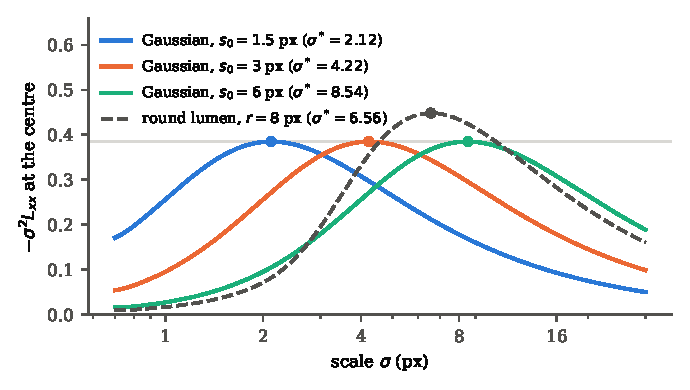
\includegraphics[width=0.72\textwidth]{fig_scale_selection.pdf}
  \caption{Scale selection with the $\sigma^2$ normalisation. Gaussian profiles of three widths peak at
  $\sigma^* = \sqrt 2\, s_0$ with the same height, $2/3^{3/2}$ (grey line). A round lumen of radius 8 px (dashed,
  normalised to the same peak) selects $\sigma^* \approx 0.8\, r$.}
  \label{fig:scale}
\end{figure}

\section{From vesselness to a graph}\label{sec:graph}

This is the Hessian baseline.
\begin{enumerate}
  \item \textbf{Centrelines.} Keep the ridge of $V$: pixels at least as high as their two neighbours across the
        vessel, $V(\x) \ge V(\x \pm \mathbf n)$, where $\mathbf n$ is the unit eigenvector of $\lambda_2$
        (non-maximum suppression, with sub-pixel interpolation).
  \item \textbf{Hysteresis.} A ridge pixel above $t_\mathrm{high}$ starts a centreline; neighbours above
        $t_\mathrm{low}$ continue it.
  \item \textbf{Graph.} Link ridge pixels into curves. Nodes are ends (one neighbour) and branch points (three or
        more). Prune spurs shorter than about one vessel width.
  \item \textbf{Widths} along each centreline from $\sigma^*$, through the calibration of
        section~\ref{sec:width}.
\end{enumerate}

\section{Where the Hessian chain fails}\label{sec:limits}

$\mathcal H_\sigma$ is a symmetric $2 \times 2$ matrix: it has one pair of axes, so it can describe \emph{one}
orientation per pixel. Where two vessels meet, that is not enough. Figure~\ref{fig:frangi} applies the chain above
(scales 1 to 11.3 px, $\beta = 0.5$, $c$ in noise units) to a synthetic optical-density image with three
junctions.
\begin{itemize}
  \item \textbf{Two equal vessels crossing at about $90^\circ$.} At the centre both eigenvalues are large and
        negative, so the pixel looks like a blob: $V = 0.20$ there, against $1.0$ along the arms. The skeleton
        of $V > 0.5$ becomes a tangle (53 branch pixels and 6 small loops within 14 px) instead of one
        four-way node.
  \item \textbf{A fork.} The two branches stay merged in $V$ for some distance past the split, so the skeleton's
        branch point lands 14 px downstream of the true fork (the trunk is 8 px wide).
  \item \textbf{A thin vessel crossing a wide one.} Here the topology survives (four arms leave the crossing), but
        inside the wide vessel $V$ and $\sigma^*$ belong to the wide vessel: the thin vessel's width and contrast
        are not measured where it crosses.
\end{itemize}
Oriented filters (orientation scores: one response per orientation at every pixel and scale) can hold two
orientations at the same pixel, which is what junctions need. In this chain the Hessian serves as the first layer
for plain vessel stretches, scale and width, and as the baseline; oriented cells take over where vessels meet.

\begin{figure}[H]
  \centering
  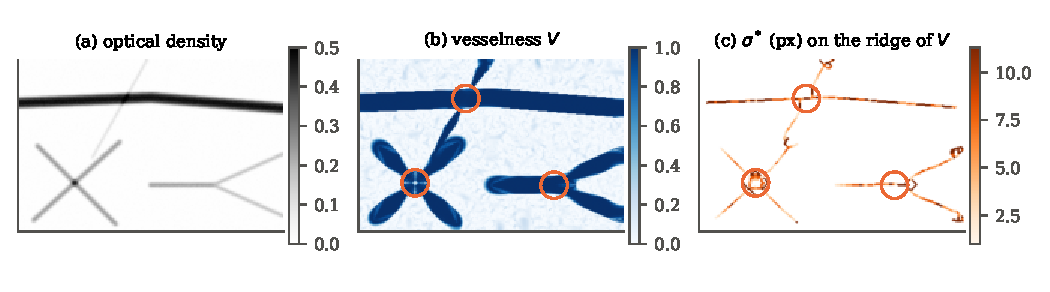
\includegraphics[width=\textwidth]{fig_frangi_example.pdf}
  \caption{Frangi vesselness on a synthetic optical-density image (round lumens, blur 1.2 px, noise 0.01): a thin
  vessel crossing a wide one (top), two equal vessels crossing (bottom left), and a fork (bottom right).
  (a) The optical density. (b) Vesselness $V$; it falls to 0.20 at the centre of the equal crossing.
  (c) The selected scale $\sigma^*$ on the skeleton of $V > 0.5$; wide vessels select larger scales. Circles mark
  the junctions.}
  \label{fig:frangi}
\end{figure}

\section*{References}
\begin{itemize}[leftmargin=*]
  \item A.~F.~Frangi, W.~J.~Niessen, K.~L.~Vincken and M.~A.~Viergever. Multiscale vessel enhancement filtering.
        \emph{MICCAI}, 1998.
  \item T.~Lindeberg. Edge detection and ridge detection with automatic scale selection. \emph{International
        Journal of Computer Vision} 30(2), 1998.
  \item M.~Guizar-Sicairos, S.~T.~Thurman and J.~R.~Fienup. Efficient subpixel image registration algorithms.
        \emph{Optics Letters} 33(2), 2008.
\end{itemize}

\end{document}
